\chapter{Introduction} 
\label{ch:introduction}

Mathematical and statistical have long been used to describe or summarize observations in genetics and genomics.
Mostly without addressing the underlying biological mechanisms mutation, selection, and drift shaping DNA sequences, but as phenomelogical description.
However, as researchers learn more about the underlying processes and more genetic and genomic data is available, the mathematical descriptions that allow us to extract information from this data have to keep up.
For example, after the unreaveling of the degenerate genetic code by \citet{MatthaeiAndNirenberg1961,NirenbergAndMatthaei1961,Maxwell1962,LederAndNirenberg1964}, and many others, researchers noticed that synonymous codons are not found in uniform proportions \citep{fitch1976,grantham1980,ikemura1981,grantham1981,sharp1988}.
Models of codon usage, however, where long purley describtive and heuristic \citep{ikemura1981,BennetzenAndHall1982,sharp1987,wright1990}.
Similarly, phylogenetic models have long been phenomelogical \citep{JukesAndCantor1969,Dayhoff1978,Kimura1980,felsenstein1981,Altschul1991}, describing the rate at which one state is transformed into another, without regards for the fundamental forces of evolution mutation, selection, and drift.
\citet{ZuckerkandlAndPauling1962} described the distance between hemoglobin proteins and proposed that the evolution of proteins is constant over time and between lineages before the genetic code was fully deciphered and were protein production was barely understood.
This dissertation is therefore focues on the application of mechanistic models rooted in first principles to protein coding sequences.

A wide variety of information is stored in protein and protein coding sequences, e.g. structure \citep{anfinsen1973}, mutation bias \citep{ShahAndGilchrist2011, gilchrist2015}, protein synthesis rate \citep{gilchrist2007,gilchrist2015}. 
Mechanistic models can be used extract these informations and to study the relative strength of mutation, selection, and genetic drift leading to the observed sequences.
Mechanistic models have a long standing history throughout biology \citep{loreau1998,DavisAndPelsor2001,adf2007}. 
They provide insights into the processes and estimates of paramerers shaping the data we observe.
In the case of this dissertation, mechanistic models lead to an understanding of the contributions of mutation, selection and drift on the evolution of observed sequences.
This allows us to use this information to learn more about these seqeunces.

\begin{figure}[H]
     \centering
	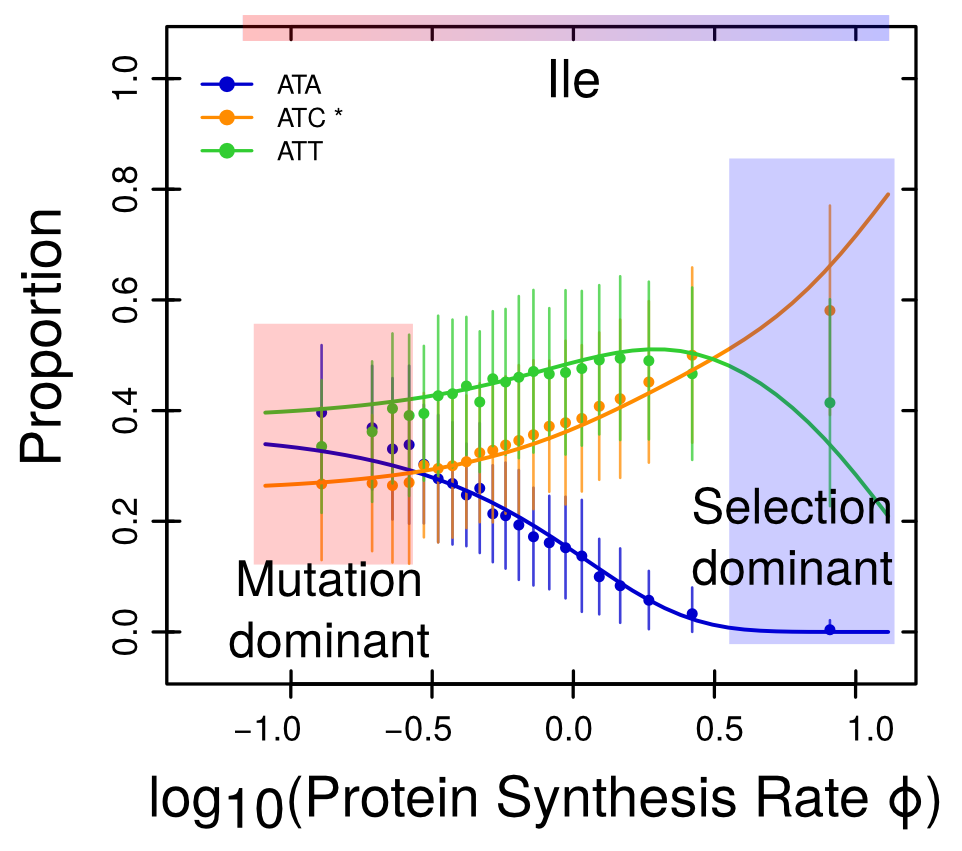
\includegraphics[width=0.6\textwidth]{ch1/expl_model}
	\caption{}
	\label{fig:expl_model}
\end{figure}

\section{Decomposing Codon Usage}

Mutation bias in codon usage is a reflection of the cellular environment while selection on codon usage allows us to make inferences about the cellular and external evironment a genome and its genes are exposed to.
The relative strength of mutation and selection on individual genes varies, allowing us to separate the effects of mutation bias and selection, specifically selection against translation overhead cost.
Genes with low protein synthesis rates are thought to be under weak selection and their codon usage is therfore dominated by mutation bias.
In contrast, genes with high protein synthesis rate are thought to be under strong selection and their codon usage is therfore dominated by selection.
However, mutation bias and selection can differ within the genome.
For example, strand specific mutation rates, differences in the tRNA pool thorughout life stages or introgressions can produce or reflect of mutliple genomic environments.
To provide researchers with a software tool, AnaCoDa \cite{landerer2018}, to address intra genomic variation in codon usage, chaper \ref{ch:anacoda} extends the mechanistic model ROC-SEMPPR \cite{gilchrist2015} to allow for a mixture distribution of mutation and selection parameters.
However, there is a significant difference to classical mixutre approaches as ROC-SEMPPR not only estimates population specific paramerers (mutation and selection) that are now modelled as mixture distibutions but also a gene specific parameter (protein synthesis rate). 
Therefore, the protein synthesis rate has to be estimated for each population, providing aditional insight into the adaptiveness of a gene to alternative genomic environments.

In chaper \ref{ch:kluyveri}, I apply AnaCoDa to the yeast \kluyveri which experienced a large scale introgression replacing the whole left arm of chromosome C.
Applying a mechanistic models allowed me to separate the effects of mutation and selection in the exogenous \kluyveri genes and the introgressed exogenous genes.
This information was used to determine a potential donor lineage in \gossypii, estimate a time since introgression, and estimate the genetic load the introgression introduced into the  \kluyveri genome.

\begin{figure}[H]
     \centering
	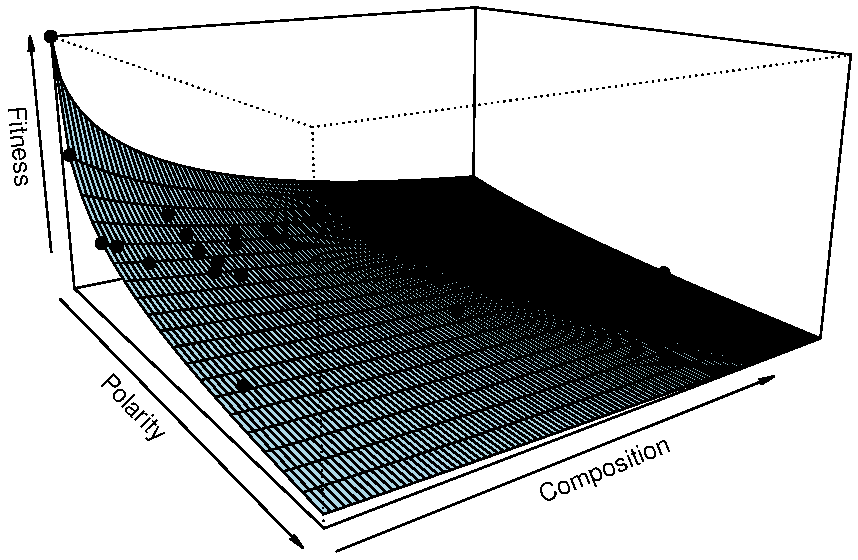
\includegraphics[width=0.7\textwidth]{ch1/decl_fitness2}
	\caption{Decline in fitness with distance in physicochemical space from the optimal amino acid. 
	Fitness decline of amino acids (black dots) relative to optimal amino acid (Alanine). Weighting of properties was obtained from \citet{grantham1974}.}
	\label{fig:decl_fit}
\end{figure}


I chapter \ref{ch:phylogeny}, I shifted my focus from the cost of protein synthesis to the functionallity or benefit a protein produces.
For that matter I utilized a mechanisitc phylogenetic model of stabilizing selection rooted in population genetics, SelAC \cite{beaulieu2018}.



% Variation in genomic environment shaping codon usage , therefore we did chapter 2.
% Applied chapter 2 to kluyveri in chapter 3
% While analysing cost of protein synthesis in chapter 3, what about protein functionality
% chapter 4 looks at protein functionality in e.coli.



%INTRODUCTION
% - Mutation, selection, drift are three main forces of evolution
% - Selection can only act on standing variation \citep{LuriaAndDelbruck1943}
% - Protein peptide sequence contains information e.g. Structure \citep{anfinsen1973}
% - Fitness effects of mutations, synonymous and non-synonymous
% -- Protein production is expensive \citep{warner1999,AkashiAndGojobori2002}
% - phylogenetics, rate of evolution \citep{ZuckerkandlAndPauling1962}

%MECHANISTIC MODELS
% - Mechanistic model can extract information on mutation and selection that describtive ones can not
% -- CAI, indifferent to mutation \citep{sharp1987}
% -- F_opt \citep{ikemura1981}
% -- CBI \citep{BennetzenAndHall1982}
% - Phylogenetic models

%INTROGRESSION
% -

%PROTEIN FUNCTIONALLITY